% Created 2013-12-08 Sun 23:44
\documentclass[11pt]{article}
\usepackage[utf8]{inputenc}
\usepackage[T1]{fontenc}
\usepackage{fixltx2e}
\usepackage{graphicx}
\usepackage{longtable}
\usepackage{float}
\usepackage{wrapfig}
\usepackage{rotating}
\usepackage[normalem]{ulem}
\usepackage{amsmath}
\usepackage{textcomp}
\usepackage{marvosym}
\usepackage{wasysym}
\usepackage{amssymb}
\usepackage{hyperref}
\tolerance=1000
\usepackage{attrib}
\usepackage{amsmath}
\usepackage{/home/evan/Documents/chicago/learning/Causality/bug}
\let\iint\undefined
\let\iiint\undefined
\usepackage{dsfont}
\usepackage[autostyle]{csquotes}
\usepackage[backend=biber,style=authoryear-icomp,sortlocale=de_DE,natbib=true,url=false, doi=true,eprint=false]{biblatex}
\addbibresource{mybibfile.bib}
\usepackage[retainorgcmds]{IEEEtrantools}
\author{Misshula, Evan\\ \texttt{Criminal Justice, CUNY Graduate Center}}
\title{Demonstration Of Instrumental Variables And Control Function Methods}
\author{Evan Misshula\\ \texttt{Criminal Justice, CUNY Graduate Center}}
\date{}
\title{Quasi-experimental design for evaluation of CURE-Violence}
\hypersetup{
  pdfkeywords={},
  pdfsubject={},
  pdfcreator={Emacs 24.3.2 (Org mode 8.2.3c)}}
\begin{document}

\maketitle





\section{Introduction}
\label{sec-1}

Violent crime is the most important social problem the policing
addresses. Violent crime remains an important public health problem in
the United States.  There were more than 9,000 gun homicides in 2008
\parencite{fbi2} and more than 71,000 non-fatal firearm injuries
\parencite{center2012injury}.  In Pittsburgh, one US city where
anti-violence programs have been implemented, young black men have a
homicide victimization rate 50x the US average \parencite{ovol2005}.

It is important to note that this problem has important secular
trends.  In the last twenty years both gun homicide and violent crime
have fallen precipitously. Gun homicide was recently 3.8 per 100K
(2010) vs 7.0 per 100K (1993) and violent crime has declined even more
sharply on a percentage basis to 2,254.2 (2010) v. 7,976.3 (1993)
\parencite{fbi1}.
\section{Model}
\label{sec-2}

\subsection{The theory of change}
\label{sec-2-1}

Cure Violence is an implementation of The Chicago Project for Violence
Prevention.  The project was conceived by Gary Slutkin
\parencite{ransford201321,slutkin2012violence} at the public health
school of the University of Illinois Chicago.  The project has a
coherent theory of change.  This theory is built on specific social
structures norms, risks and choices.  The model is novel because it
treats violence as an epidemic.  People who engage in acts of violence
are not regarded as bad people.  They are regarded as sick (or
infected by their environment).  As such it runs counter to many
established criminological theories and moral philosophy such as the
Biological
\parencite{Gibson2002,Lambroso1890,Lambroso1890a,Gould1996},
Individual Trait \parencite{glueck1950unraveling,glueck1956physique},
Self-control \parencite{Gott1990,Akers1991} and Genetic Theory of
Crime
\parencite{moffitt1993adolescence,moffitt2005new,barkan1992retreat}.
The theory also holds that as in the treatment of disease, punishment
is likely to be overvalued as a method of behavior change which sets
it apart from both Classical
\parencite{beccaria2009crimes,devine1981cesare} and Rational Choice
\parencite{becker1974crime,levitt2004understanding} Criminology.
Dr. Slutkin's previous work on HIV in Africa informs the work.  It was
during his years in Uganda that the World Health Organization was able
to reduce HIV transmission rates dramatically (Figure \ref{fig:hivdrop},
p. \pageref{fig:hivdrop}).

\begin{figure}[htb]
\centering
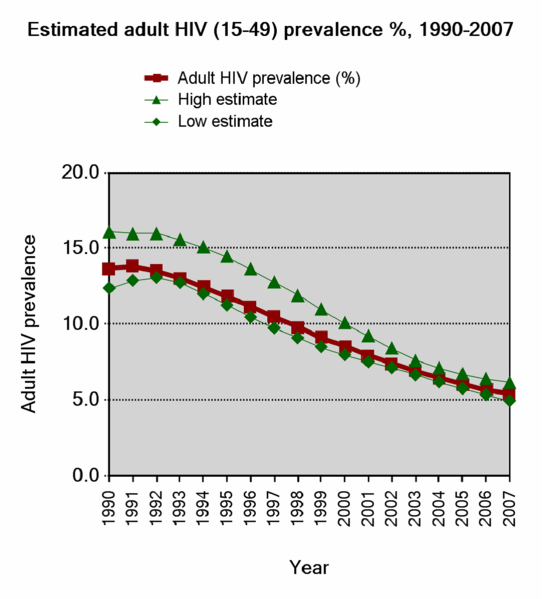
\includegraphics[width=.9\linewidth]{./assets/543px-Estimated_adult_(15-49)_HIV_prevalence,_Uganda,_1990-2007.png}
\caption{\label{fig:hivdrop}HIV prevalence in Uganda 1990-2005 \parencite{world2008epidemiological}}
\end{figure}


These social structures act as inputs.  The inputs are posited to be
causally related to violence. Designing an evaluation and testing this
theory is the point of this proposal.  The theory of the program
allows us to look at not just what participants actions are supposed
to be but also what the influence are supposed to be \parencite{Leeuw2003}.

\subsection{Mechanism}
\label{sec-2-2}

In Cure Violence the participants are encouraged to stop
shooting. Ceasefire did not demand that their clients cease all
criminal activities just that they not use deadly violence in their
disputes.  In fact, violence interuptors often reminded participants
and gang leaders that violence was bad for their ostensible business,
selling drugs.  In this way, Cure Violence can be thought of as harm
reduction not personal redemption.
\subsection{Focus on highest risk people}
\label{sec-2-3}

Client selection tried to operationalize ``high risk of being shot or being a shooter.'' 
Clients needed to be:

\begin{itemize}
\item between 16 and 15
\item a person with history of arrests and imprisonment
\item involved in drug trade
\item a gang member
\item a recent shooting victim
\end{itemize}
\subsection{Mechanism to stop shooting}
\label{sec-2-4}

The three conditions the program seeks to change are the norms for settling disputes, the 
alternatives to deadly violence to settle disputes and the perceived risk of engaging in violence.
\subsection{Causal Factors}
\label{sec-2-5}

\subsubsection{Norm Change}
\label{sec-2-5-1}

Norms define a range of behavior that most in a community find acceptable even if self-adherence is 
not perfect.  Norms vary from community to community.  If the majority in a community feel that the 
institutions of civil society are inherently biased against them they will not avail themselves of 
those institutions.  In many high crime areas people believe that crime against other persons is 
wrong and unacceptable.  However deep suspicion of the police and criminal justice system may allow a
culture of ``no snitching'' to prevail.  Cure Violence sought to restore faith in the Criminal Justice
system as an effective means of dealing with violence and disrupt the norms against talking to the 
police.

Encouraging debates over ``what people will and won't accept'' was a core strategy.  This was
done with rallies and local debates.  This was consistent with wide distribution of anti-violence
literature.
\subsubsection{Decision Alternatives}
\label{sec-2-5-2}

Violence interruptors sought to disparage violence when it would be counterproductive.  They also 
negotiated and promoted truces.  They negotiated fines and occasionally steered conflict to 
physical altercations.  This behavior severely reduced but did not eliminate injury.

\subsubsection{Risk Enhancement}
\label{sec-2-5-3}

Focus potential shooters on the consequences of their actions on the community they still have, 
their mother, siblings and grandparents.  Use the grief at gang funerals for a positive message and 
remind the potential shooter that they are not immune to the long-term consequences of gang
involvement.
\section{Evaluation}
\label{sec-3}

Evaluation of the efficacy of a program like Cure Violence poses
substantial theoretical and methodological challenges. The long
downward trend in crime creates the possibility of that this program
simply co-occurred with a decline in crime rather than caused it.
Since the intervention is not strictly randomized a comparison group
needs to be constructed.  This general methodology is called a
Quasi-experiment \parencite{shadish}.  Indeed many other explanations
for a decline in crime have been posited in the academic literature.

\subsection{Alternative explanations for the secular decline in crime}
\label{sec-3-1}

Alternative mainstream explanations for the decline in crime include
the increased number of people in prison
\parencite{levitt2004understanding}, more effective police deterrence
\parencite{braga2008pulling}, better police tactics
\parencite{capowich1995evaluating}, and an older population
\parencite{van2004criminal}. More offbeat ideas include more abortion
\parencite{donohue2001impact} and less exposure to lead paint
\parencite{nevin2000lead}.  Yet the last time American Academy of
Science commissioned a review of the literature it found no definitive
cause \parencite{blumstein2008factors}.
\subsection{Prior evaluations of Cure Violence}
\label{sec-3-2}

There have been four cities who have released prior evaluations of
Cure Violence
\parencite{skogan2008evaluation,webster2009interim,wilson2010community,picard2013testing}.
The methodologies used have become increasingly sophisticated in terms
of isolating causality and correcting for various confounding biases
such as selection bias.  Design differences are summarized in Table
\ref{tab:design} (p. \pageref{tab:design}) and estimation differences
in Table \ref{tab:estimation} (p. \pageref{tab:estimation}).

\begin{center}
\begin{tabular}{lrlll}
\hline
City & Year & Comparison & Spatial & Outcome\\
\hline
Chicago & 2008 & 2 Police Beats & Geo & V Pos\\
Baltimore & 2010 & 1 Neighborhood & None & Pos\\
Pittsburgh & 2010 & Whole City & Spillover & No effect\\
Brooklyn & 2012 & 3 precincts & None & Pos\\
\hline
\end{tabular}
\end{center}
\begin{center}
\begin{tabular}{lrlll}
\hline
City & Year & DiD & Correction & Outcome\\
\hline
Chicago & 2008 & No & None & V Pos\\
Baltimore & 2010 & Yes & None & Pos\\
Pittsburgh & 2010 & Yes & Propensity & No effect\\
Brooklyn & 2012 & Yes & None & Pos\\
\hline
\end{tabular}
\end{center}


\section{Suitable comparison tracts will be selected by}
\label{sec-4}
matching Cure Violence areas with tracts with similar demographic
features. The matching variables included racial composition, family
organization, poverty, number of young men, unemployment and home
ownership.

A prior evaluation of the program used a conventional Box-Jenkins-Tiao
intervention analysis with a transfer function at the start of the
intervention.  As per Box and Tiao (1976) a difference of means test
between the actual number and the predicted number of shootings during
program operation.  Kernel Density Estimation was used to detect
change in spatial patterns of crime over time.

\subsection{Comparison Sites}
\label{sec-4-1}

In Chicago for the prior evaluation each site had between two and four
comparison sites. In NYC, there are 2 sites operational with 2 more
funded to open.  Each new site will be restricted to a single census
tract. The evaluation team has been given data (under strict
non-disclosure and non-dissemination from the New York Police
Department "NYPD").  NYC is composed 2166 census tracts.  We received
data on homicide in 1130 census tracts, arrests for violent crimes in
745 census tracts, complaints of violent crimes in 792 census tracts
and shootings in 1348 census tracts. Negotiation with the NYPD for
more complete data is ongoing.

The approach of the prior evaluation was to use a limited number of
``best matches''.  This appears to waste information that may be
contained in the non ``k-best'' matches.  We would propose to create a
distribution of matches from all non-program and non-competing program
sites by examining the similarity of the crime over time.  The crime
data rather than the demographics should take precedence in
constructing the comparison.  Missing data should be imputed through
multiple imputation.  An ARIMA model has the form:

\begin{equation}
Y_t=f(X_t)+N_t
\end{equation}

The intervention is designated \( I_t \).  Enumerating the ARIMA(p,d,q) model:

\begin{equation}
\Delta^d y_t = \mu + \phi_1 \Delta^d y_{t-1} + \phi_2 \Delta^d y_{t-2} + \cdots + \phi_p \Delta^d y_{t-p} + \\
\theta_{t-1} \epsilon_{t-1} + \theta_{t-2} \epsilon_{t-2} + \cdots + \theta_{t-q} \epsilon_{t-q}
\end{equation}

where \( \epsilon_t \sim N(0, \sigma^2_{\epsilon}) \).  Time series analysis follows a standard protocol:

\begin{enumerate}
\item Perform a Dickey-Fuller test for stationarity
\item Check for seasonality, and if so, correct for it
\item Check for the presence of an integrated trend
\item Estimate the noise parameters
\item Check impact speed and duration
\end{enumerate}

This is not appropriate for homicide because of the censoring problem at 0.  In this case we will attempt a
poisson regression and use negative binomial if variance is significantly greater than the mean.
\subsection{Spatial inequality in the risk of crime over time}
\label{sec-4-2}

Kernel Density estimation has been used to create heat maps before and after an intervention.  Prior 
evaluations have used a negative exponential density with a half mile grid.  Also it is possible to
create an inequality of spatial risk of crime.  By using ordered crime index data we can also create a
Lorenz Curve shooting risk.  This allows us to calculate both overall and time weighted gini coefficients 
for each crime category.
\section{References}
\label{sec-5}

\printbibliography[heading=none]
% Emacs 24.3.2 (Org mode 8.2.3c)
\end{document}